\documentclass[../main.tex]{subfiles}
\graphicspath{{\subfix{../images/}}}

\setcounter{secnumdepth}{0}
\begin{document}

\section{3. domácí úlohy}

\subsection{1a)}
\subsubsection*{Zadání}
Buď $G=(V,E)$ $k$-regulární bipartitní graf s částmi $L$ a $R$. Dokažte, že $|L|=|R|$.

\subsubsection*{Řešení}

Počet hran vycházejících z $L$ je zřejmě $k |L|$, počet hran vycházejících z $R$, je zřejmě $|k|R$.

Je zřejmé, že se oba tyto výrazy musí rovnat (jedná se o 2 různé způsoby jak spočíst všechny hrany v grafu), proto tedy $|L| = |R|$
\qed


\subsection{1b)}
\subsubsection*{Zadání}
Nalezněte, až na isomorfismus, všechny bipartitní grafy $G$, jejichž doplněk $\bar{G}$ je též bipartitní.

\subsubsection*{Řešení}

Po provedení doplňku se z $L$ a $R$ stanou úplné podgrafy. Vezměme tedy třeba úplný podgraf $\bar{L}$, 
pokud je $|L|>2$ určitě by v něm existoval lichý cyklus. 
Protože podgraf bipartitního grafu musí být také bipartitní dostáváme, že
$|L|, |R| \leq 2$. 

Z tohoto plyne, že aby pro  graf $G=(V,E)$ platilo, že jeho doplněk je bipartitní tak pak $|V|\leq 4$.

Navíc také platí, že mezi každou trojicí vrcholů musí být buď 1 nebo 2 hrany. V opačném případě existuje v grafu nebo jeho doplňku lichý cyklus.

Z toho plyne že $G$ nemůže být prázdný/úplný pro $|V|\geq 3$.

Pro případ $|V| = 4$ tedy dostáváme následující grafy:

Jako množinu vrcholů vezměme $[4]$. 

BÚNO (jinak by šlo pouze o izomorfismus) má graf  hranu $\{1,2\}$. 
Mezi vrcholy $2,3,4$ ale není žádná hrana, kvůli předchozímu tvrzení musíme mezi nimi jednu hranu přidat.
Máme 2 možnosti (kvůli izomorfismu) buď přidáme hranu $\{2,3\}$ nebo $\{3,4\}$  $(\star)$.

Pro případ $\{2,3\}$, ale opět chybí hrana mezi $1,3,4$, hranu $\{1,3\}$ přidat nemůžeme, vznikl by cyklus o délce 3. Proto přidáme 
hranu například $\{3,4\}$ (druhá možnost je opět izomorfní s touto). Doplněk tohoto grafu je pak izomorfní se sebou samým. Rozdělení které existuje je $L = \{1,3\}, R = \{2,4\}$.

Nakonec bychom k tomuto grafu ještě mohli přidat hranu $\{4,1\}$, vznikl by cyklus, doplněk tohoto grafu by byl izomorfní s grafem s hranami  $\{1,2\}, \{3,4\}$ (tímto jsme se dostali k $(\star)$, navíc z grafu s hranami $\{1,2\}, \{3,4\}$ dostaneme přidáním libovolné hrany graf isomorfní s předchozím případem).
Tento graf je i se svým doplňkem opět bipartitní, volme například $L = \{1,3\}, R = \{2,4\}$.


Případ $|V| = 3$:

Jako množinu vrcholů vezměme $[3]$. 

BÚNO má graf  hranu $\{1,2\}$. Přidáním další hrany dostaneme jeho doplněk a oba tyto grafy jsou bipartitní.

Případ $|V| = 2$:

Prázdný graf je zřejmě bipartitní, jeho doplněk je $G=([2], {1,2})$ je také.

Případ $|V| = 1,0$:

Oba dva tyto degenerované případy jsou bipartitní a jsou doplňkem sebe sama. 

Na obrázku můžeme vidět všechny grafy s jejich doplňky (bez degenerovaných případů). 
Obarvení určuje rozdělení do $L$ a $R$

\begin{figure}[!h]
    \centering
    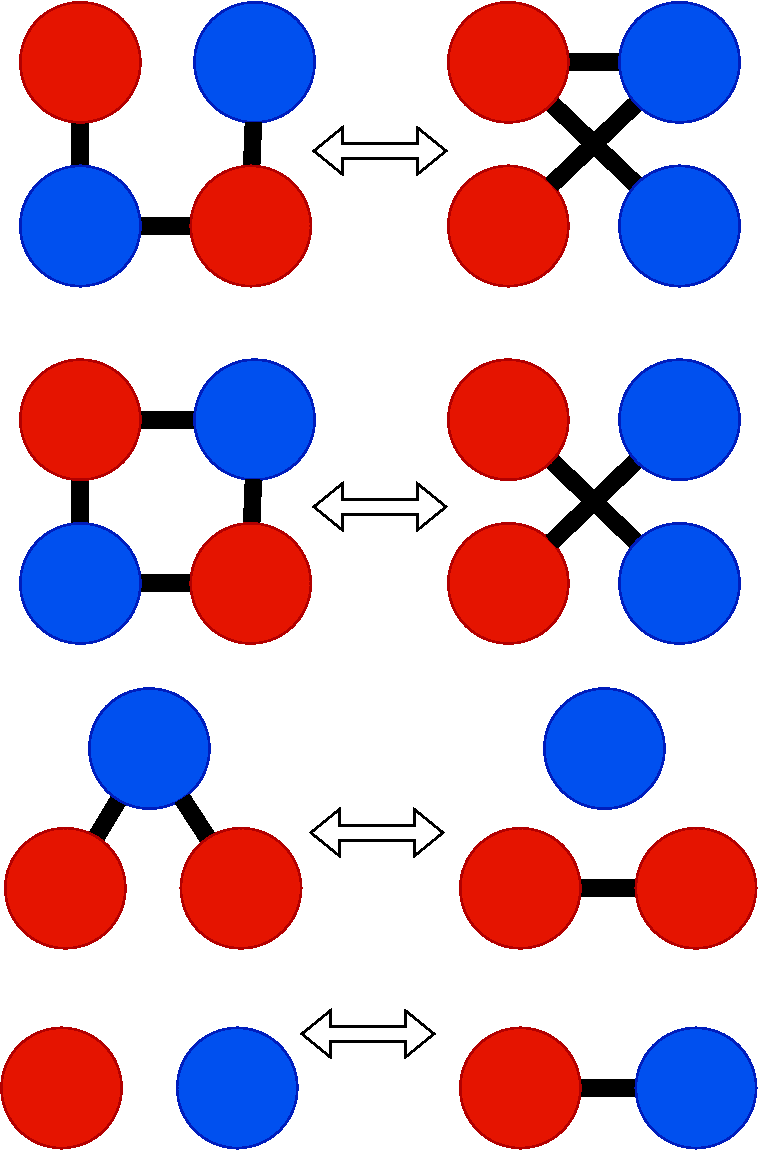
\includegraphics[height=\linewidth]{images/BipartiteComplement.pdf}
    \caption*{Všechny bipartitní grafy jejichž doplněk je také bipartitní}
\end{figure}






\subsection{2)}
\subsubsection*{Zadání}
Pro graf $G=(V,E)$ označme průměrem $G$ maximální délku nejkratší cesty mezi nějakými dvěma vrcholy, tzn. $\max_{u,v\in V} \text{dist}_{G}(u,v)$. Dokažte, že má-li graf průměr alespoň 4, tak jeho doplněk má průměr nejvýše 2.

\subsubsection*{Řešení}

Pokud by graf měl více než jednu komponentu souvislosti tvrzení by pak bylo triviální, každý vrchol má totiž pak v sousedství všechny vrcholy z ostatních komponent, tj. nejkratší cesta mezi každými dvěma body je nejvýše 2.

Řešme tedy případ s jednou komponentou souvislosti.

Protože graf má průměr $\geq4$ určitě obsahuje cestu nejkratší délky přesně 4, stačí z nejdelší nejkratší cesty vzít libovolné 4 po sobě jdoucí vrcholy.

Označme vrcholy cesty jako $v_1, ... v_5$, pak musí platit, že v grafu neexistují následující hrany
\begin{equation*}
    \{v_1,v_3\},\{v_1,v_4\},\{v_1,v_5\},\{v_2,v_4\},\{v_2,v_5\},\{v_3,v_5\}
\end{equation*}

Navíc neexistují vrcholy $w,u\notin\{v_1,v_2,v_3,v_4,v_5\}$, pro který by existovala nějaká dvojice následujících hran (platí i pro $u$).

\begin{equation*}    
\left\{\{v_1, w\}, \{w, v_4\}\right\},
\left\{\{v_1, w\}, \{w, v_5\}\right\},
\left\{\{v_2, w\}, \{w, v_5\}\right\},
\end{equation*}

Navíc nemohou existovat následující 2 trojice $\left\{\{v_1, w\}, \{w,u\}, \{u, v_5\}\right\}$ nebo $\left\{\{v_1, w\}, \{w,u\}, \{u, v_5\}\right\}$.

Všechny tři tyto omezení plynou z toho, že $v_1,...,v_5$ tvoří nejkratší cestu mezi $v_1$ a $v_5$.

Provedeme  doplněk:

Z druhého omezení plyne, že pro $\forall w,u \notin \{v_1,v_2,v_3,v_4,v_5\}$,
máme vždy alespoň jednu z každé dvojice hran, navíc existuje jedna z hran z každé trojice z třetího omezení. 

Například tedy existuje  jedna z hran $\left\{\{v_1, w\}, \{w, v_5\}\right\}$ a 
jedna z hran $\left\{\{v_1, u\}, \{u, v_5\}\right\}$. 

Ukažme sporem, že toto implikuje, že mezi uzly $u,w$ existuje 
nejkratší cesta délky nejvíce 2.

\begin{proof}
    Předpokládejme, že taková cesta neexistuje.

    Zřejmě tedy musí platit, že pro libovolné $v\in\{v_1,...,v_5\}$ nemůže existovat dvojice hran $\left\{\{w,v\},\{v,u\}\right\}$, poté by totiž cesta určitě existovala.

    Díky této podmínce dostaneme BÚNO (stačilo by přeznačit $u,w$) 
    z první dvojice následující hrany $\{v_1, w\}, \{u, v_4\}$.

    Z druhé dvojice máme jedinou možnost jak hrany zvolit a to $\{v_1, w\}, \{u, v_5\}$.

    Z třetí dvojice máme opět jedinou možnost, a to jsou  hrany $\{v_2, w\}$, $\{u, v_5\}$.

    Máme tedy hrany $\{v_1, w\}, \{v_2, w\}, \{u, v_4\}, \{u, v_5\}$. 

    Nakonec z třetího omezení máme $\left\{\{v_1, u\}, \{w,u\}, \{w, v_5\}\right\}$
    existence libovolné hrany z této trojice je ale spor.
     
\end{proof}
V doplňku tedy existuje cesta délky 2 mezi každými vrcholy, které nejsou součástí cesty.

Zabývejme se nyní vrcholy na cestě.

Z prvního omezení triviálně plyne, že vrcholy $v_1, v_3, v_5$  a $v_2, v_4$,
tvoří úplné grafy, jsou od sebe tedy vzdálenost 1. 

Navíc díky první a druhé podmínce platí, že tyto
vrcholy jsou ve vzdálenosti 2 od libovolného vrcholu mimo cestu.\\
Například pro vrchol $v_1$ máme z druhé podmínky existenci jedné z 
hran $\left\{\{v_1, w\}, \{w, v_4\}\right\}$ a z první podmínky máme v doplňku hranu $\{v_1,v_4\}$, 
z toho plyne zřejmě plyne, že buď existuje cesta $v_1, w$ nebo cesta $v_1, v_4, w$.\\
Stejně můžeme postupovat i pro vrcholy $v_2, ... , v_5$

% Z $(\star)$ také platí, že $dist(v_1,v_2) = 2$ a $dist(v_4,v_5) = 2$

Chybí nám ukázat vzdálenosti mezi $v_1,v_2$, mezi $v_4,v_5$, mezi $v_1, v_4$, mezi $v_5, v_2$, mezi $v_2, v_3$ a mezi $v_3, v_4$.

To opět plyne z prvního omezení.

Triviálně pro $v_1, v_4$ a $v_5, v_2$.

Pro $v_2, v_3$ volíme cestu procházející přes $v_5$, pro $v_3, v_4$ procházející přes $v_1$.

Tím jsme ukázali, že pokuď má graf průměr alespoň 4, tak jeho doplněk má průměr nejvýše 2.
\qed




\subsection{3)}
\subsubsection*{Zadání}
Pro graf $G=(V,E)$ označme $g(G)$ délku nejkratšího cyklu, který $G$ obsahuje; pokud je $G$ acyklický, definujeme $g(G)\coloneq \infty$.
Poznamenejme, že parametru $g(G)$ se také říká obvod grafu.

Buď $d\geq 3$ a $r\geq 2$ pevné a $G=(V,E)$ libovolný $d$-regulární graf. Dokažte
\begin{enumerate}
    \item Je-li $g(G)=2r$, tak  potom $|V| \geq \frac{2(d-1)^r -2}{d-2}$
    \item Je-li $g(G) = 2r + 1$ tak potom $|V|\geq \frac{d(d-1)^r -2}{d-2}$
\end{enumerate}

\subsubsection*{Řešení}


\subsection{4)}
Připomeňme, že pro graf $G=(V,E)$ nazveme hranu $e\in E$ mostem, jestliže podgraf $(V,E\setminus\{e\})$ má více komponent souvislosti než $G$.\\
Analogicky nazveme vrchol $v\in V$ artikulací, jestliže indukovaný podgraf množinou $V\setminus{v}$ má více komponent souvislosti než $G$.

\subsection{4a)}
\subsubsection*{Zadání}
Dokažte, že každý $2k$- regulární graf neobsahuje most.
\subsubsection*{Řešení}

BÚNO mějme souvislý graf. 

$k = 1$:
\begin{lemma*}
    Pro 2-regulární souvislý graf platí, že každý vrchol je součástí cyklu. 
\end{lemma*}
\begin{proof}
    Mějme libovolně velký souvislý 2-regulární graf. 
    Zvolme vrchol $v$ s jeho sousedy $w,u$, 
    na tyto vrcholy klademe podmínku, že netvoří cyklus o délce 3. 
    
    Z tohoto grafu vyrobme menší graf tím, že odstraníme vrchol $v$ a přidáme hranu $\{w,u\}$, tím jsme dostali menší graf, touto operací určitě nezanikne žádný cyklus, zároveň pokud je uzel $w$ v cyklu v novém grafu tak byl uzel $v$  v cyklu v původním grafu. 
    
    Tuto operaci můžeme opakovat dokud nedostaneme graf s 3 vrcholy. Protože se jedná o 2 regulární graf tak se musí jednat o cyklus. 
\end{proof}

Z toho plyne, že každý $2$-regulární graf neobsahuje  most. 

$k>1$:






\subsection{4b)}
\subsubsection*{Zadání}
Dokažte, že každý $k$-regulární bipartitní graf neobsahuje artikulaci.

\subsubsection*{Řešení}

Z 1a) víme, že  $|L|=|R|$. BÚNO mějme souvislý graf. 

Pro $k=1$ je tvrzení triviální, máme graf $G=([2], \{1,2\})$, odebráním vrcholu dostaneme $G=([1], \emptyset)$ což je stále jedna komponenta.

Uvažujme $k=2$: 

Z lemmatu dokázaného pro 4b) víme, že každý vrchol v 2-regulárním grafu je součástí cyklu, 
odstraněním jednoho vrcholu z cyklu určitě nedostaneme novou komponentu souvislosti.

$k\geq 3$:

Vezměme 




\subsection{5a)}
\subsubsection*{Zadání}
Buď $G=(V,E)$ neprázdný graf a buď $d \coloneq \frac{|E|}{|V|}$. 
Dokažte, že $G$ obsahuje indukovaný podgraf $H$ splňující $\delta(H) > d$.

(Nápověda: zkuste z $G$ postupně odebírat vrcholy stupně nejvýše $d$.)

\subsubsection*{Řešení}

Postupujme podle nápovědy. Vezměme graf $G_i = (V_i, E_i)$ a 
odeberme z něj vrchol stupně nejvýše $d_i \coloneq \frac{|E|}{|V|}$, tím vytvoříme graf $G_{i+1}$

Platí, že $d_i \leq d_{i+1}$. Toto plyne z \todo{Upravit}
\begin{equation*}
    \frac{|E_i|}{|V_i|} \leq \frac{|E_{i+1}|}{|V_{i+1}|} = \frac{E_{i} - \frac{|E_i|}{|V_i|}}{|V_i| - 1} 
\end{equation*}

Toto opakujeme, dokud se nedostaneme do situace, kdy v grafu není vrchol, který by měl stupeň menší než $d_i$.\\
Tím dostáváme graf, kde máme alespoň $n$ vrcholů nejméně stupně $d_i$, což jsme chtěli ukázat. 


\subsection{5b)}
\subsubsection*{Zadání}
Pro každé přirozené $d\geq 1$ a každé $\varepsilon\in(0,1)$ zkonstruujte graf $G_{d,\varepsilon}= (V,E)$
takový, že splňuje $\frac{|E|}{|V|} > d - \varepsilon$ a 
zároveň $\delta(H)\leq d$ pro každý podgraf $H \subseteq G_{d,\varepsilon}$.


\subsubsection*{Řešení}

Vezměme $i$-regulární graf $G$ o $2n$ vrcholech ($i<2n$).
Z handshaking lemmatu pak dostaneme, že $2|E| = 2in$. Odeberme z něj jednu hranu a máme 

\begin{equation*}
    |E| = in - 1
\end{equation*}

% V dalším kroku konstrukce vezměme $n$ grafů $G$. Vytvořme nový nesouvislý graf $H$, 
% kde každé $G$ je jedna z jeho komponent souvislosti.
% Tento graf má zřejmě $|V| = 2n$ vrcholů.\\
% Dále jednoduše dostáváme, že $G$ má 
% \begin{equation*}
%     |E| = n(\frac{ik}{2} - 1)
% \end{equation*} 
% hran. 
Z toho máme, 
\begin{equation*}
    \frac{|E|}{|V|} = \frac{i}{2} - \frac{1}{2n}
\end{equation*}

$i$ zvolme tak, aby platilo $i = d$. 

$2n$ můžeme zvolit libovolně velké a proto tedy existuje $n$ tak, že člen $\frac{1}{2n} < \varepsilon$ pro libovolné $\varepsilon$.

Navíc, protože graf má sudý počet vrcholů tak víme, že existuje (plyne z první série úkolů).

Tímto jsme sestrojili graf, který splňuje $\frac{|E|}{|V|} > d - \varepsilon$. 

Protože je ale původní graf je $i$-regulární/$d$-regulární, tak i každý jeho indukovaný podgraf je nejvíce $d$-regulární.

\end{document}